\subsection{Primary Flow Diagram}
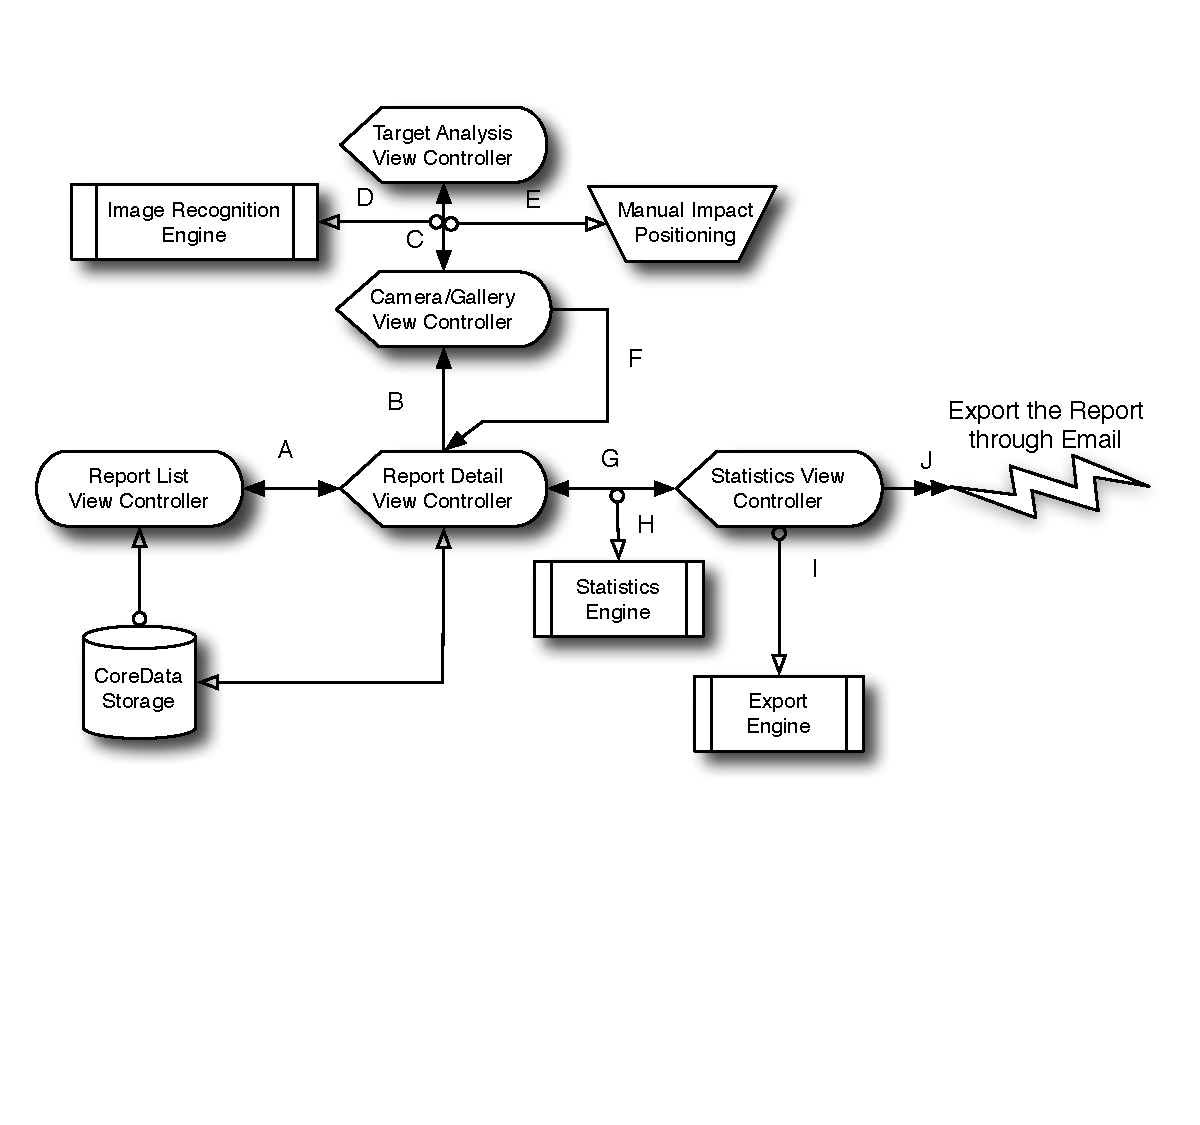
\includegraphics[width=.91\textwidth]{ArchitectureModel20.pdf}

\subsubsection{Description of Primary App Flows}
\paragraph{A.} This flow goes from the master view controller to the test detail view controller which will show the detail view of a stored test. This is the basic test information. Statistical Report information will be shown on another screen.
\paragraph{B.} This flow shows what happens when the user chooses to edit the photo associated with the app. Another view is presented to give the user the option to view the current photo or change the photo.
\paragraph{C.}  If the user chooses to replace the current photo they are given the option to take a new photo or use an image in the photo gallery. This is the flow for the photo gallery view. The user is presented with their standard photo gallery and can choose an image before clicking done. If the user presses analyze then the image is reanalyzed in another view which first makes and attempt at finding all of the holes (D) and then give the user a chance to correct, add, and/or remove holes (E).
\paragraph{F.} The user is sent back to the Report Detail View Controller.
\paragraph{G.} The user can click a ``Export'' button to be taken to the Report Detail View Controller. This controller creates the report for the test including all statistical calculations. Report generation is handled this way to ensure that a user can not send and out of date report from the app over email. A new report is generated every time from the data in the test. 
\paragraph{H.} The Report Statistics Engine handles calculating the statistical information from the points given in the photo. It then passes this data back to the Test Report View Controller for viewing.
\paragraph{I.} The Report Export Engine handles generating the report file that will be emailed off of the device. 
\paragraph{J.} This is the CSV plus Image file being sent through Email.

\subsubsection{Description of Supplementary App Flows}
\paragraph{} In addition to the main application controllers there will need to be a few supplementary controllers. They are described below.
\paragraph{1.} \textbf{Picker View Controllers} Any time a Picker view is used in the interface there will have to be another view controller to handle the Picker view. 

\newpage
\subsection{User Interface Screen Shots}
\subsubsection{Main App Screen}
\begin{figure}[H!htb]
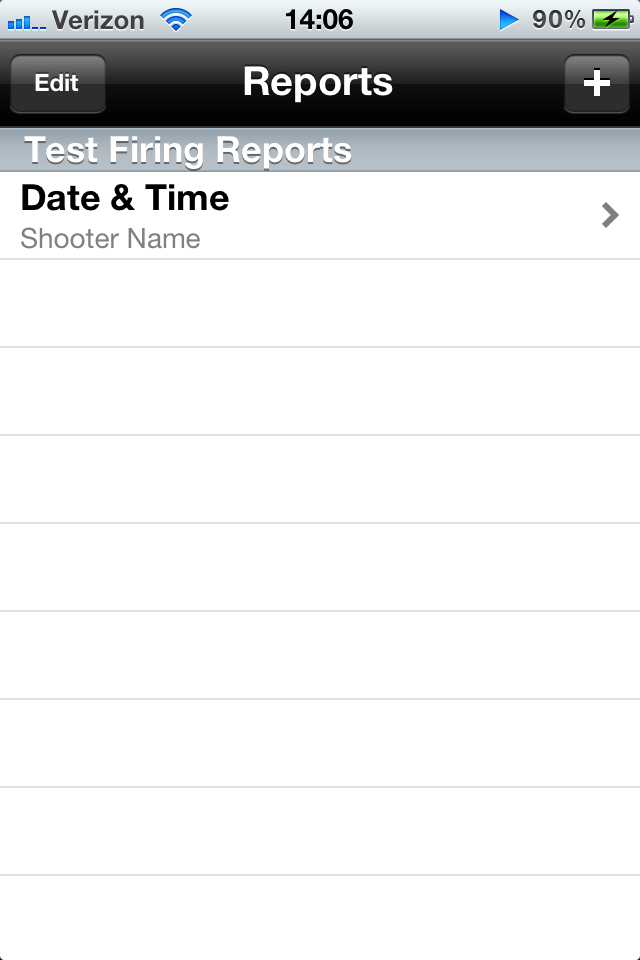
\includegraphics[width=3in]{ScreenShots111011/MainPage.png}
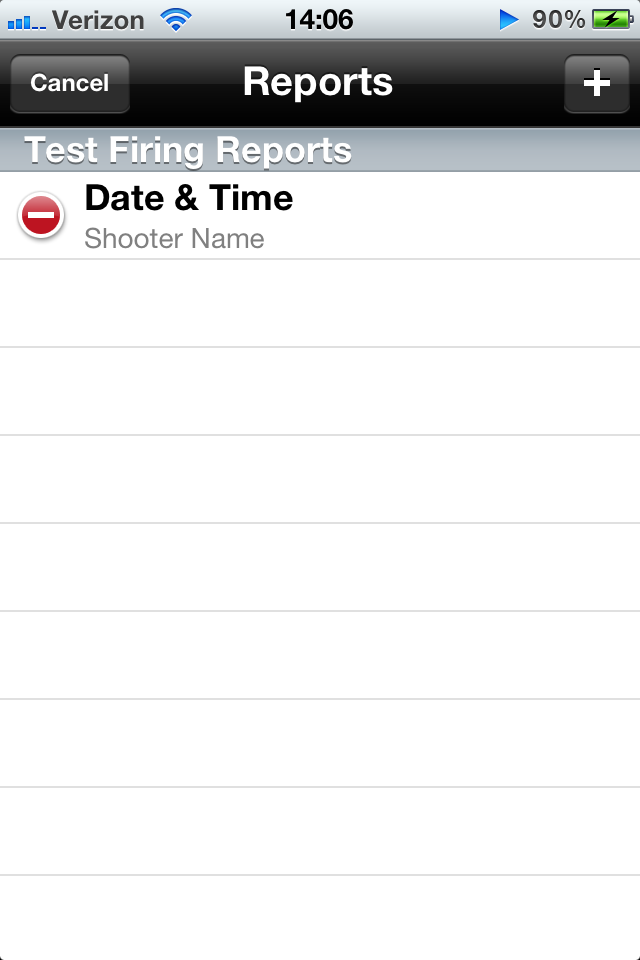
\includegraphics[width=3in]{ScreenShots111011/MainPageEdit.png}
\begin{minipage}{0.5\linewidth}
\caption{This is the view controlled by the Master View Controller in its normal mode.}
\end{minipage}
\begin{minipage}{0.5\linewidth}
\caption{This is the view controlled by the Master View Controller when it is in editing mode.}
\end{minipage}
\end{figure}

\newpage
\subsubsection{New Test Screen}
\begin{figure}[H!htb]
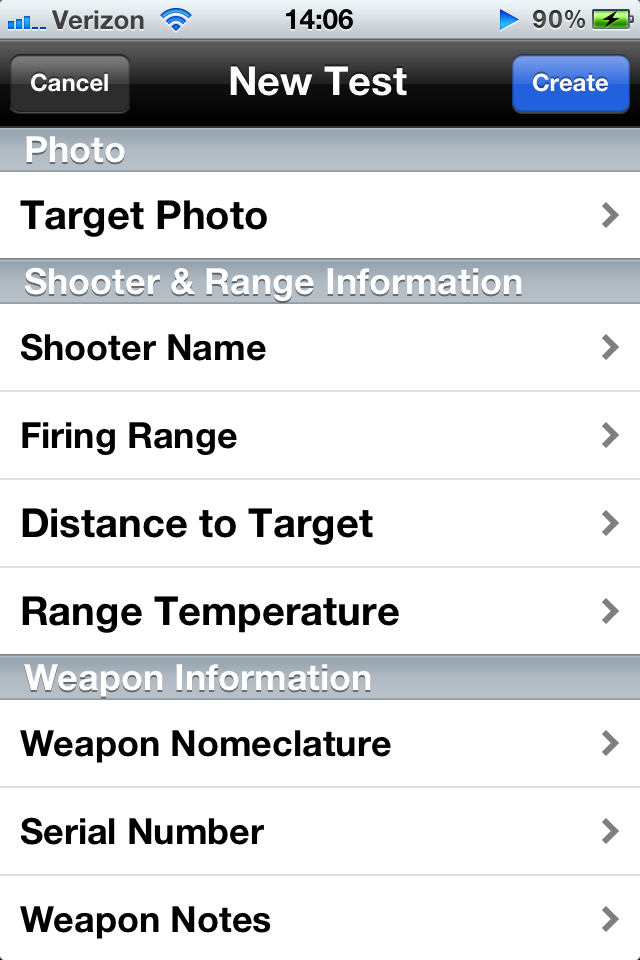
\includegraphics[width=3in]{ScreenShots111011/NewTest.png}
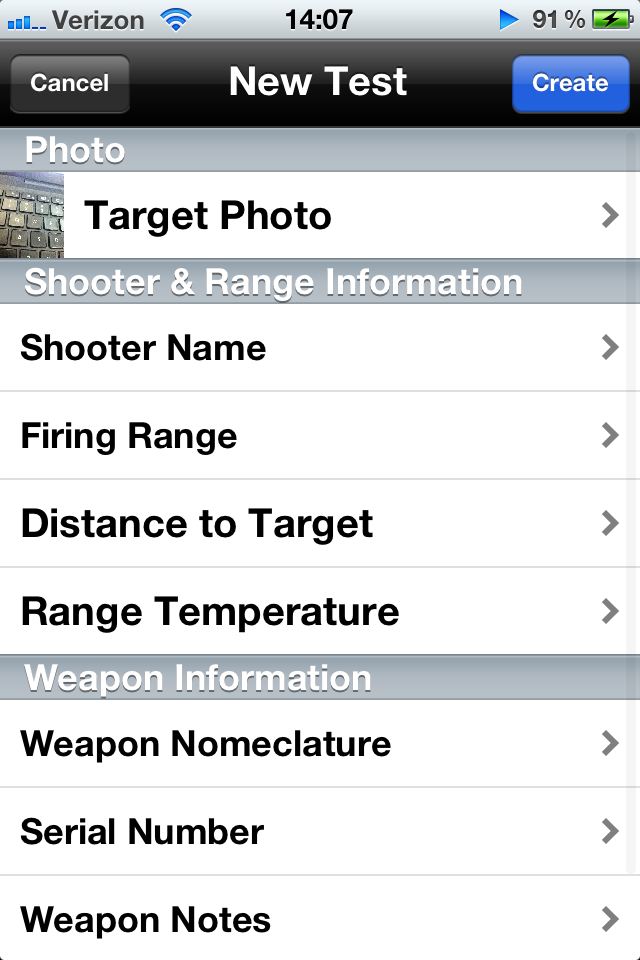
\includegraphics[width=3in]{ScreenShots111011/NewTestPhoto.png}
\begin{minipage}{0.5\linewidth}
\caption{This is the view controlled by the New Test View Controller without a picture associated with the test.}
\end{minipage}
\begin{minipage}{0.5\linewidth}
\caption{This is the view controlled by the New Test View Controller with a picture associated with the test.}
\end{minipage}
\end{figure}

\newpage
\subsubsection{Take Photo Screen}
\begin{figure}[H!htb]
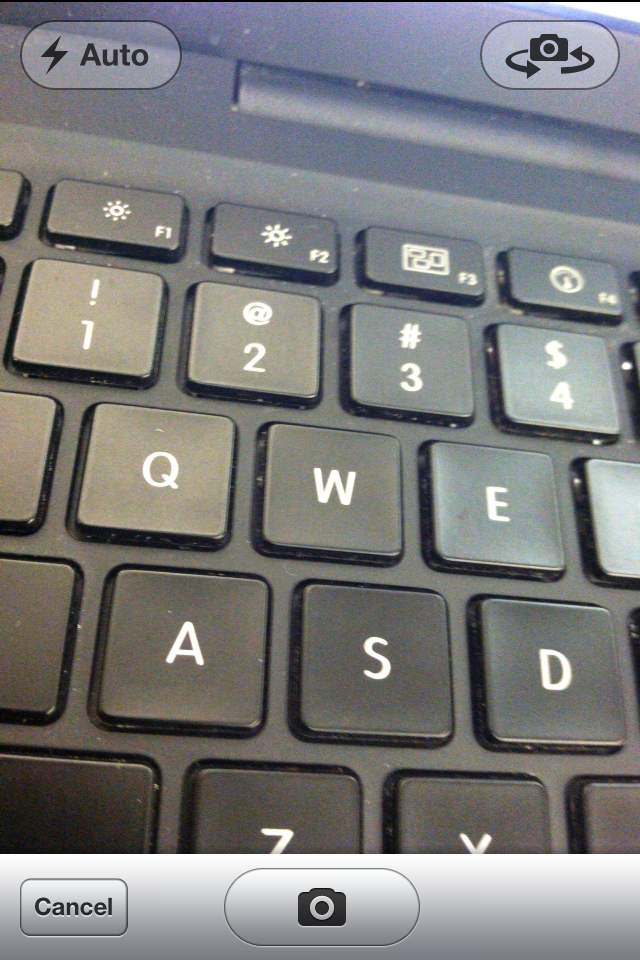
\includegraphics[width=3in]{ScreenShots111011/TakePhoto.png}
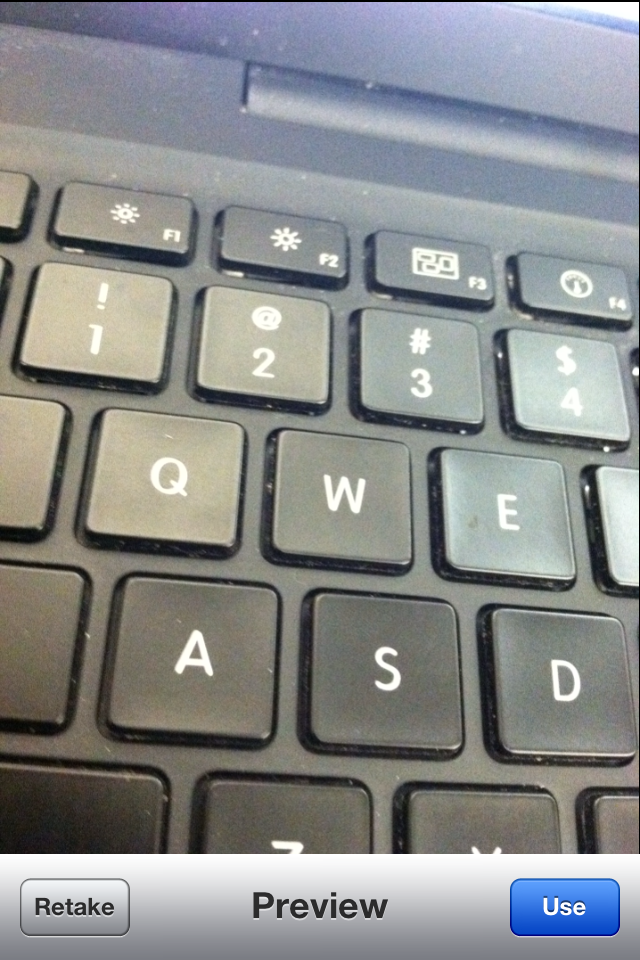
\includegraphics[width=3in]{ScreenShots111011/RetakePhoto.png}
\begin{minipage}{0.5\linewidth}
\caption{This is the camera screen, which is native to the device, before an initial image it taken.}
\end{minipage}
\begin{minipage}{0.5\linewidth}
\caption{This is the camera screen, which is native to the device, when the retake/use image option is presented}
\end{minipage}
\end{figure}

\newpage
\subsection{Video Demo}

\begin{figure}[H!htb]
\centering
\includemovie[text=(Click to Load Video...),mouse=true,controls,url]{1.0\textwidth}{0.6\textwidth}{http://www.halldjack.com/storage/iSANTAFirstUserInterfacePrototype.mp4}
\caption{The video will only play if you are viewing this document in Acrobat Reader or another pdf viewer that supports multimedia playback. You can also view this video \href{http://youtu.be/dN2K_zHrJ9M}{\color{blue}Here}}
\end{figure}

%\newpage
\subsection{System Background}
\paragraph{} This will include a brief description on how the different pieces of the architecture will be tied together.
\paragraph{} First because we are using the Model, View, Controller paradigm every view will have a view controller. These view controllers will handle all of the functional logic for the view. These views will pass control along with any necessary information between each other as the user changes views. This is helpful because each view becomes very modular and can be moved around and reused very easily.
\paragraph{} The view controllers will be backed up by a few engines where they are needed. The engines are designed to hide some of the complex algorithms from the view controllers. Anywhere that we do complex tasks, such as normalizing an image, we will move the logic in to an engine. This helps to simplify the view controller code along with giving us an easier way to be able to test these algorithms.
\paragraph{} By using these tactics we are going to have a very modular system that will be easy to expand and easy to track bugs down in. This should help speed up development.
\paragraph{} Because storing Tests is a key feature we have put a lot of research in to determining which of the methods available in iOS development is the most advantageous for our application. We have decided to use Core Data which is a built in SQLlite-esque database. It does not have many of the features of a Database Management system. However it does allow us to use relations and multiple entities as well as export a test as an xml object which will aide our conversion to a report that is printable from a computer.
\begin{figure}[H!htb]
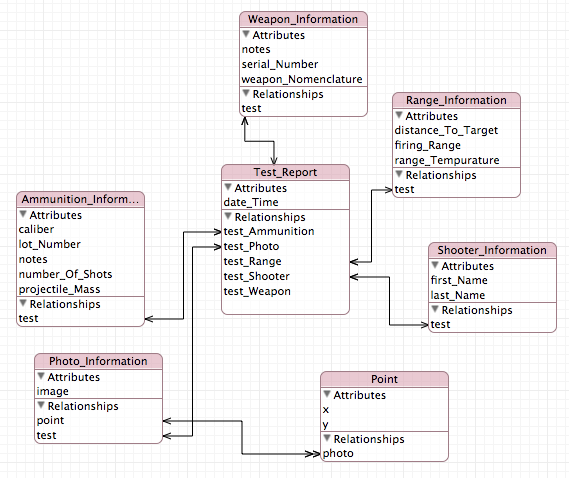
\includegraphics[width=5in]{CoreDataModel.png}
\caption{This is a depiction of our Core Data Model. It shows the entities, their relations, and the attributes of each entity.}
\end{figure}
